\documentclass[tikz,border=10pt]{standalone}
\usepackage{amsmath}
\usetikzlibrary{trees, positioning, arrows.meta, calc}

% Define the requested color
\definecolor{darkyelloworange}{RGB}{230, 150, 0}

\begin{document}

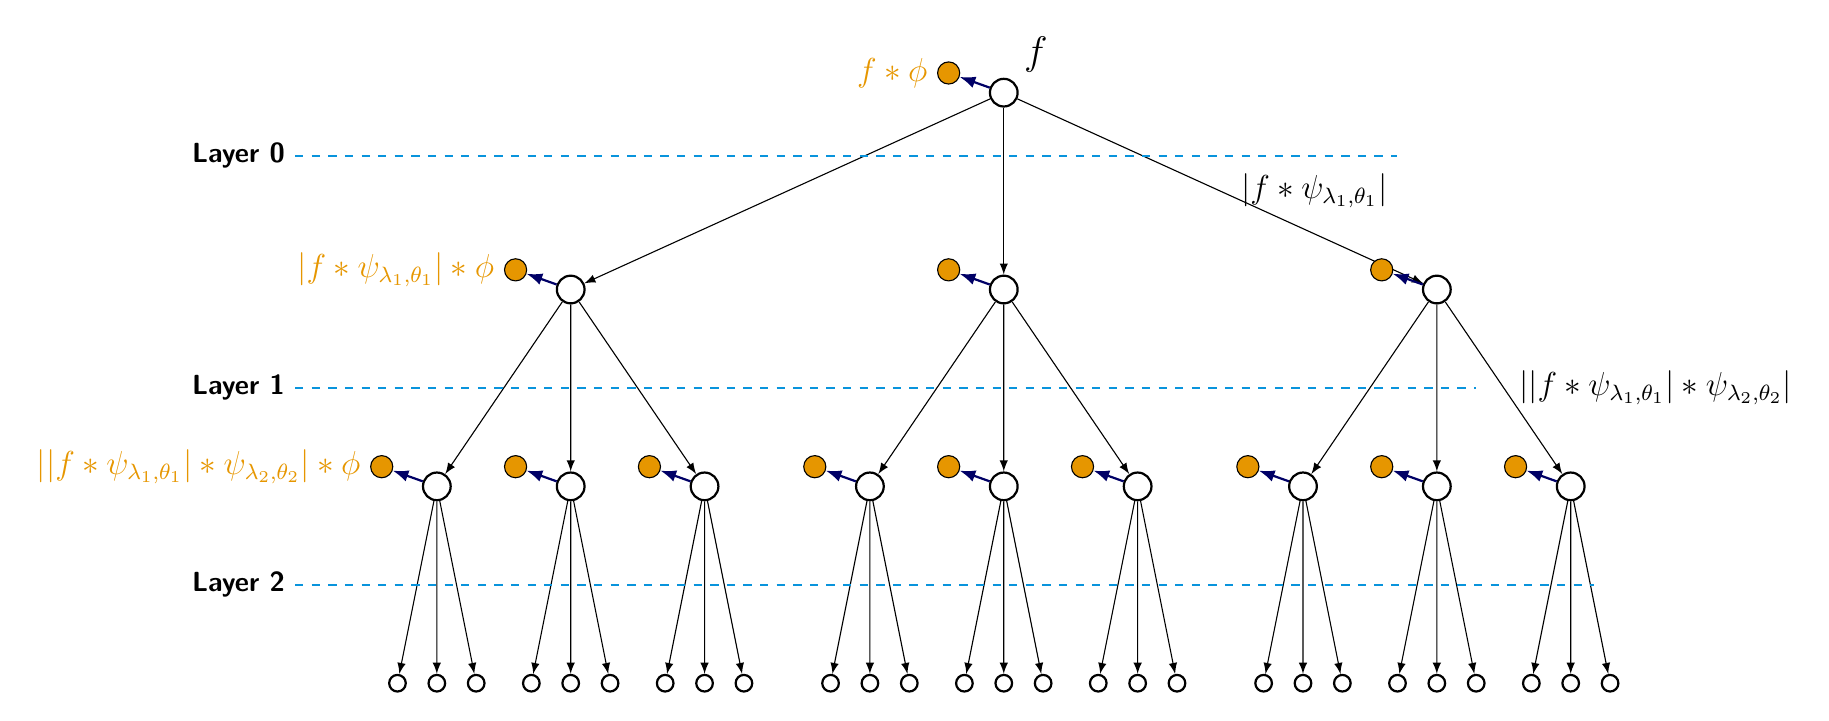
\begin{tikzpicture}[
    % Node Styles
    wnode/.style={circle, draw=black, thick, fill=white, inner sep=0pt, minimum size=10pt},
    % Updated style with new color
    rnode/.style={circle, draw=black, fill=darkyelloworange, inner sep=0pt, minimum size=8pt},
    leaf/.style={circle, draw=black, thick, fill=white, inner sep=0pt, minimum size=6pt},
    % Edge Styles
    edge from parent/.style={draw, -latex, thin},
    bluearrow/.style={-{Latex[length=2mm]}, color=blue!40!black, thick},
    layerline/.style={dashed, color=cyan!80!blue, thick},
    % Tree Spacing
    level 1/.style={sibling distance=5.5cm, level distance=2.5cm},
    level 2/.style={sibling distance=1.7cm, level distance=2.5cm},
    level 3/.style={sibling distance=0.5cm, level distance=2.5cm}
]

% Draw the main tree structure
\node[wnode, label={[font=\Large\bfseries, anchor=south west]45:$f$}] (root) {}
    child { node[wnode] (L1-1) {}
        child { node[wnode] (L2-1) {} child {node[leaf]{}} child {node[leaf]{}} child {node[leaf]{}} }
        child { node[wnode] (L2-2) {} child {node[leaf]{}} child {node[leaf]{}} child {node[leaf]{}} }
        child { node[wnode] (L2-3) {} child {node[leaf]{}} child {node[leaf]{}} child {node[leaf]{}} }
    }
    child { node[wnode] (L1-2) {}
        child { node[wnode] (L2-4) {} child {node[leaf]{}} child {node[leaf]{}} child {node[leaf]{}} }
        child { node[wnode] (L2-5) {} child {node[leaf]{}} child {node[leaf]{}} child {node[leaf]{}} }
        child { node[wnode] (L2-6) {} child {node[leaf]{}} child {node[leaf]{}} child {node[leaf]{}} }
    }
    child { node[wnode] (L1-3) {}
        child { node[wnode] (L2-7) {} child {node[leaf]{}} child {node[leaf]{}} child {node[leaf]{}} }
        child { node[wnode] (L2-8) {} child {node[leaf]{}} child {node[leaf]{}} child {node[leaf]{}} }
        child { node[wnode] (L2-9) {} child {node[leaf]{}} child {node[leaf]{}} child {node[leaf]{}} }
    };

% Helper macro for side nodes (formerly red nodes)
% #1: Parent Node Name, #2: Label Text (optional)
\newcommand{\addSideNode}[2]{
    \node[rnode] (r-#1) at ($(#1) + (-0.7, 0.25)$) {};
    \draw[bluearrow] (#1) -- (r-#1);
    \ifx&#2&\else
        % Updated text color to match the node
        \node[anchor=east, text=darkyelloworange, font=\large] at (r-#1.west) {#2};
    \fi
}

% Add Side Nodes and Labels
% Root
\addSideNode{root}{$f * \phi$}

% Level 1
\addSideNode{L1-1}{$|f * \psi_{\lambda_1, \theta_1}| * \phi$}
\addSideNode{L1-2}{}
\addSideNode{L1-3}{}

% Level 2
\addSideNode{L2-1}{$||f * \psi_{\lambda_1, \theta_1}| * \psi_{\lambda_2, \theta_2}| * \phi$}
\foreach \i in {2,...,9} {
    \addSideNode{L2-\i}{}
}

% Edge Labels (Rightmost path)
\path (root) -- (L1-3) node[midway, right=4pt, font=\large] {$|f * \psi_{\lambda_1, \theta_1}|$};
\path (L1-3) -- (L2-9) node[midway, right=2pt, font=\large] {$||f * \psi_{\lambda_1, \theta_1}| * \psi_{\lambda_2, \theta_2}|$};

% Layer Lines and Labels
% Layer 0 moved up from -1.25 to -0.8
\draw[layerline] (-9, -0.8) node[left, text=black, font=\sffamily\bfseries] {Layer 0} -- (5, -0.8);
\draw[layerline] (-9, -3.75) node[left, text=black, font=\sffamily\bfseries] {Layer 1} -- (6, -3.75);
\draw[layerline] (-9, -6.25) node[left, text=black, font=\sffamily\bfseries] {Layer 2} -- (7.5, -6.25);

\end{tikzpicture}
\end{document}